\documentclass[dvips,12pt]{article}
\usepackage[left=0.65in,top=0.3in,right=0.65in,bottom=0.3in]{geometry} % Document margins
% Any percent sign marks a comment to the end of the line

% Every latex document starts with a documentclass declaration like this
% The option dvips allows for graphics, 12pt is the font size, and article
%   is the style

\usepackage[pdftex]{graphicx}
\usepackage{url}
	
% These are additional packages for "pdflatex", graphics, and to include
% hyperlinks inside a document.

\setlength{\oddsidemargin}{0.25in}
\setlength{\textwidth}{6.5in}
\setlength{\topmargin}{0in}
\setlength{\textheight}{8.5in}

% These force using more of the margins that is the default style

\begin{document}
	
	% Everything after this becomes content
	% Replace the text between curly brackets with your own
	
	\title{Keyword Extraction by Deep Learning \\Mid Term Report}
	\author{Yi Cheng(yicheng1), Anoop Hallur(ahallur), Xiaoqiu Huang(xiaoqiuh)}
	\date{\today}
	
	% You can leave out "date" and it will be added automatically for today
	% You can change the "\today" date to any text you like
	
	\maketitle
	
	% This command causes the title to be created in the document
	
	\section{Introduction}
	
		As the goal of our project, we plan to do keyword extraction using deep learning. We are aiming to improve the performance of keyword extraction by deep learning techniques as compared to other techniques used previosuly.
		We believe that Deep learning techniques can improve the performance because when it has been applied to other similar tasks, a significant improvement has been observed.
		For example , Google speech recognizer uses Deep Neural Networks and accuracy is extremely high[cite].The area of applying deep learning to keyword extraction has not been explored much, hence we are trying to apply it and see how it performs.
	\section{Related Work}
	
		Before diving into the details of our model and algorithm, we want to summarize the related work that has been done in the field of Keyword Extractions, how they can be applied to our project and how deep learning can be applied to solve this particular problem and our thoughts on why deep learning should give better performance compared to other algorithms.
		
		\subsection{Baseline Algorithms of Keyword extraction}
		
		A survey was done by Lott.B[cite], and he summarizes that whenever he have a large corpus of data already available(as in our case), TF-IDF is the most accurate algorithms of the existing ones. 
		
		In TF-IDF model, we assign weight to each term in the model, and we choose the top'n' weighted words as the keywords for the text. The weight of each word is computed by taking into account the Term Frequency(TF) and Inverse Domain Frequency(IDF), where Term Frequency indicates how significant is the term to a spcicif document, and IDF takes into account how common the word is in the domain. We have implemented the benchmarks for this algorithms on our dataset.
		
		Other algorithms presently being used are some variant of TF-IDF with domain specific modifications. For example , one technique uses a Bayes classifier with TF-IDF to compute the weights and extract the keywords. 
		There are techniques which are to be used when we dont have a corpus of text available to us. Frequency based single Document Keyword Extraction is one such technique. This techniques coputes word weights by measuring the frequency of text occurence within two punctuation marks in the text. Since we have text corpus available, we did not want to be compared against these classes of algorithms.
		\subsection{Deep Learning Intution}
	\section{Model Description}
	
	\section{Experiment and Results}
		\subsection{Baseline Algorithm Results}
		
		To evaluate the performance of our approach compared to existing techniques, we have used Precision and Recall rates as our benchmarking standards.
		We have formally defined these parameters as 
		
		$Precision = \frac{ sizeof(A \bigcap B)}{sizeof(A)}$
		
		$Recall    = \frac{ sizeof(A \bigcap B)}{sizeof(A)}$
		
		where A is the set of predicted tags and B is the set of actual tags.
		
		We have implemnted TF-IDF and Bayseian Classifier approach as described by the survey for Keyword Extraction on our data set. With plain vanilla TF-IDF, the average precision and recall rates were less than 10 \%. However, after preprocessing the data by using a stemmer, the accuracy is a modest 15-20\% on topics in our data set for as the best performer.
		We have used portland stemmer, available as part of open source NLTK(Natural Language Processing Toolkit) project.
		The Bayesian Classifier is similar to TF-IDF apporach except that it takes into account the position of the word in text. The weight of each term is reduced as the log of the its position from the begining of the sentence.
		
		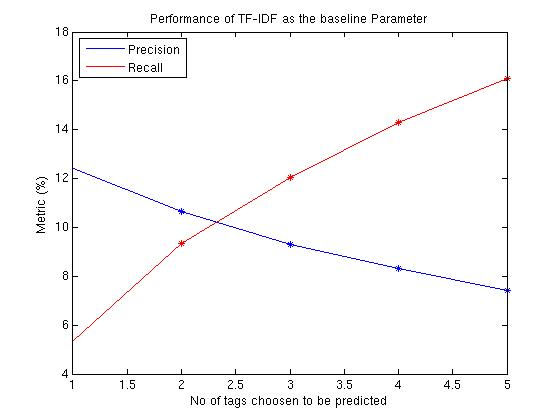
\includegraphics[width=0.5\textwidth]{../baseline/TfIdf.jpg}
		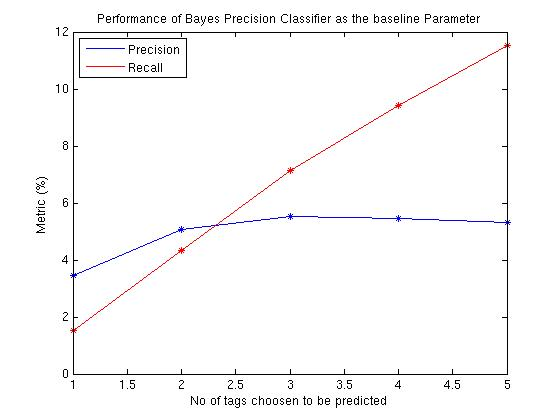
\includegraphics[width=0.5\textwidth]{../baseline/BayesPrecisionClassifier.jpg}
				
		As part of survey paper[6], we found out that the existing standard for key word extraction uses Lexical Tree approach and we are coming up with the precision and recall rates for Lexical Trees approach \\\{Report exact figures here\}.
		
		\subsection{Dataset}
		
		We had identified data from stackexchange( \url{https://archive.org/download/stackexchange/stackexchange_archive.torrent}) to be a suitable data set for our project. 
		
		Of the 20 GB, available to us, for the feasibility of the experiment, we are using only 95 MB of data, on about 5 topics for our evaluation. Although the data set seems to be small compared with original one, we felt this was enough for testing purposes. Later we will try to \textbf{increase the data set} when our model is finished.
        
        Here is an interesting question, why we choose several topic and not only one topic as small data set to test our model? In fact we did that, but found that it's not a good way to do testing of the task like keyword extraction. For a single topic, some words will occur frequently, for example, in the topic of \emph{apple}, the words like \emph{osx} and \emph{iphone} will occur frequently in most documents which according to \emph{tf-idf}, they are not important words. But in fact they are the tags for many documents in this topic. And if we train the model on only a single dataset, then if the model only predict the top frequently tags, it can still gain good performance. That's the reason we use several topics as dataset here.
        \subsection{Our Model}
        Our work is based on the open source software \footnote{https://github.com/sancha/jrae}. For the midterm report, we use the tool to do some simple checking and we also modify some parts of the it to make use of the word vectors generated by \emph{word2vec}\footnote{https://code.google.com/p/word2vec/}, another tool developed by Google.
        
        Before discussing about the experiment, we will introduce the method about training data preprocessing. For now, the model is a supervised model,  
	\section{Pending Work}
	

	% An article style is separated into sections and subsections with 
	%   markup such as this.  Use \section*{Principles} for unnumbered sections.
	\section{References}
    \begin{enumerate}
        \item Bengio Y, Schwenk H, Senécal J S, et al. Neural probabilistic language models[M]//Innovations in Machine Learning. Springer Berlin Heidelberg, 2006: 137-186.
        \item Socher R, Perelygin A, Wu J Y, et al. Recursive deep models for semantic compositionality over a sentiment treebank[C]//Proceedings of the Conference on Empirical Methods in Natural Language Processing (EMNLP). 2013: 1631-1642.
        \item Socher R, Lin C C, Manning C, et al. Parsing natural scenes and natural language with recursive neural networks[C]//Proceedings of the 28th International Conference on Machine Learning (ICML-11). 2011: 129-136.
        \item Collobert R, Weston J, Bottou L, et al. Natural language processing (almost) from scratch[J]. The Journal of Machine Learning Research, 2011, 12: 2493-2537.
        \item Matsuo Y, Ishizuka M. Keyword extraction from a single document using word co-occurrence statistical information[J]. International Journal on Artificial Intelligence Tools, 2004, 13(01): 157-169.
        \item Lott B. Survey of Keyword Extraction Techniques[J]. UNM Education, 2012.
        \item Hasan K S, Ng V. Automatic Keyphrase Extraction: A Survey of the State of the Art[J].
    \end{enumerate}
\end{document}